\section{Algorithms}
\label{sec:algo}



\subsection{Distance from Nearest Walls}

Geometric information can be botained from measuring Round Trip Time (RTT)
of a probing chirp. 

\subsubsection{Chirp}


sweep frequency chirp


Select Chirp Amplitude and Frequency

We firstly measure the ambient sound, and choose a quiet frequency.


What is chirp


why chirp?


How to generate chirp?


What chirp to use?


How to see echo? Time delay of echo, Shape of echo pulse, Phase Diff


SNR etc.

\fxnote{GRAPH: chirp and echo shape}

\subsubsection{Recording}

\subsubsection{Cross-correlation and Audio Reduction}

After receiving the original sound and echo, we do auto-correlation with original sound,
and remove it from the audio track.

\fxnote{GRAPH: how auto-correlation works}


\subsubsection{Locating Echoes}

Envelop is the sound of big surface. Physical explanation. 
Define envelop as the same duration of original sound.



\begin{figure}[H]
\centering
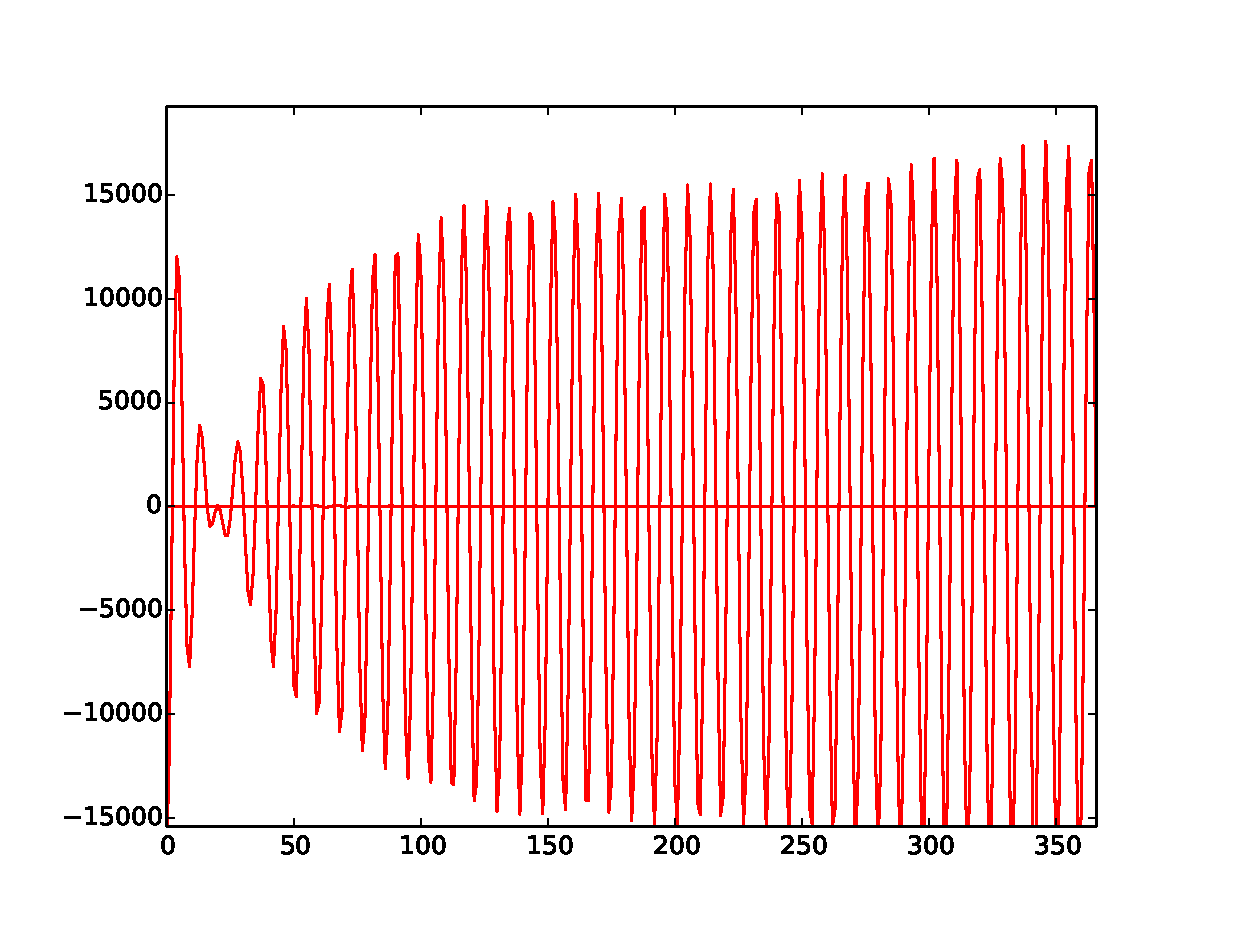
\includegraphics[width=0.45\textwidth]{./fig/20cm.eps}
\caption{20cm from wall, 50ms chirp}
\end{figure}

\begin{figure}[H]
\centering
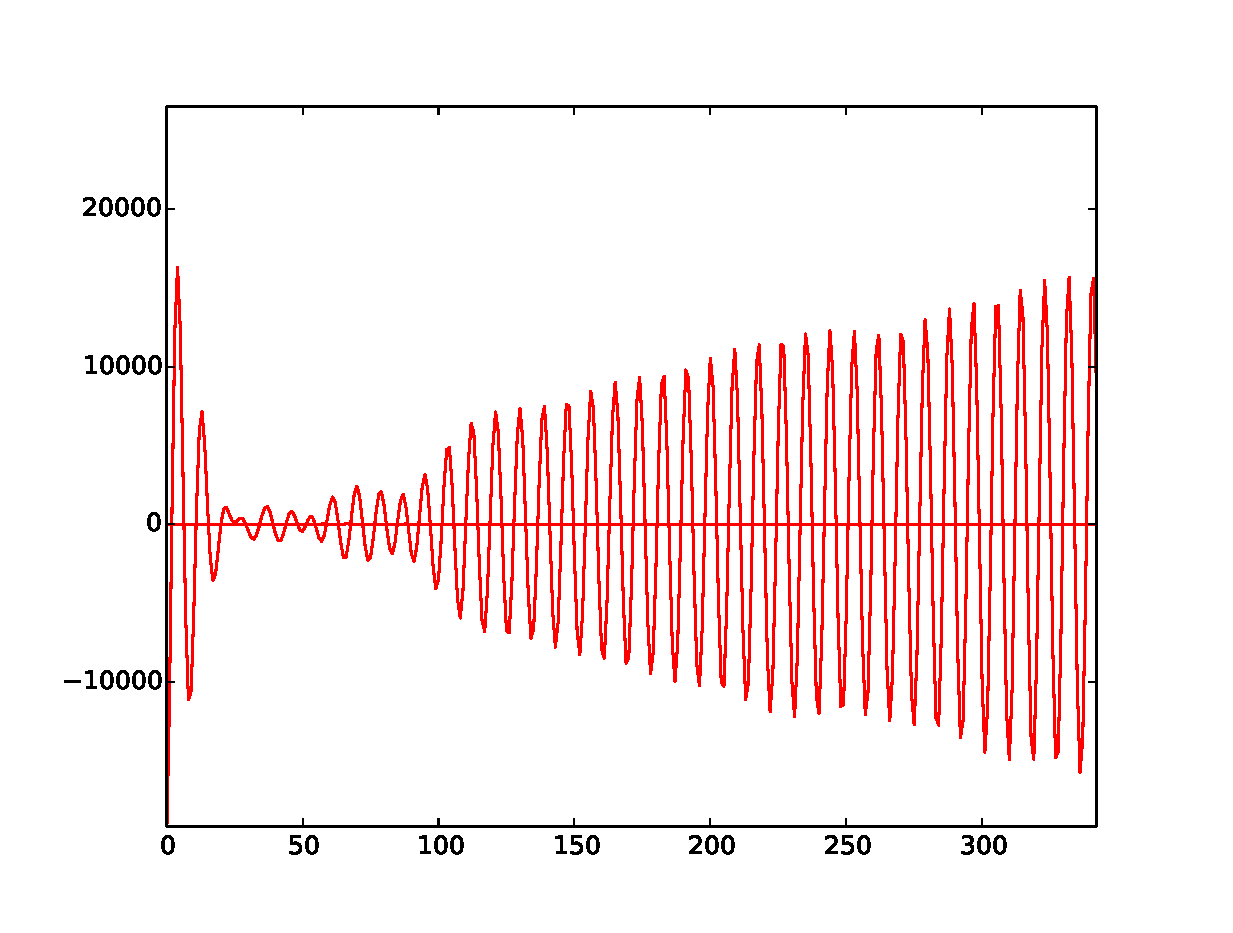
\includegraphics[width=0.45\textwidth]{./fig/40cm.eps}
\caption{40cm from wall, 50ms chirp}
\end{figure}

\begin{figure}[H]
\centering
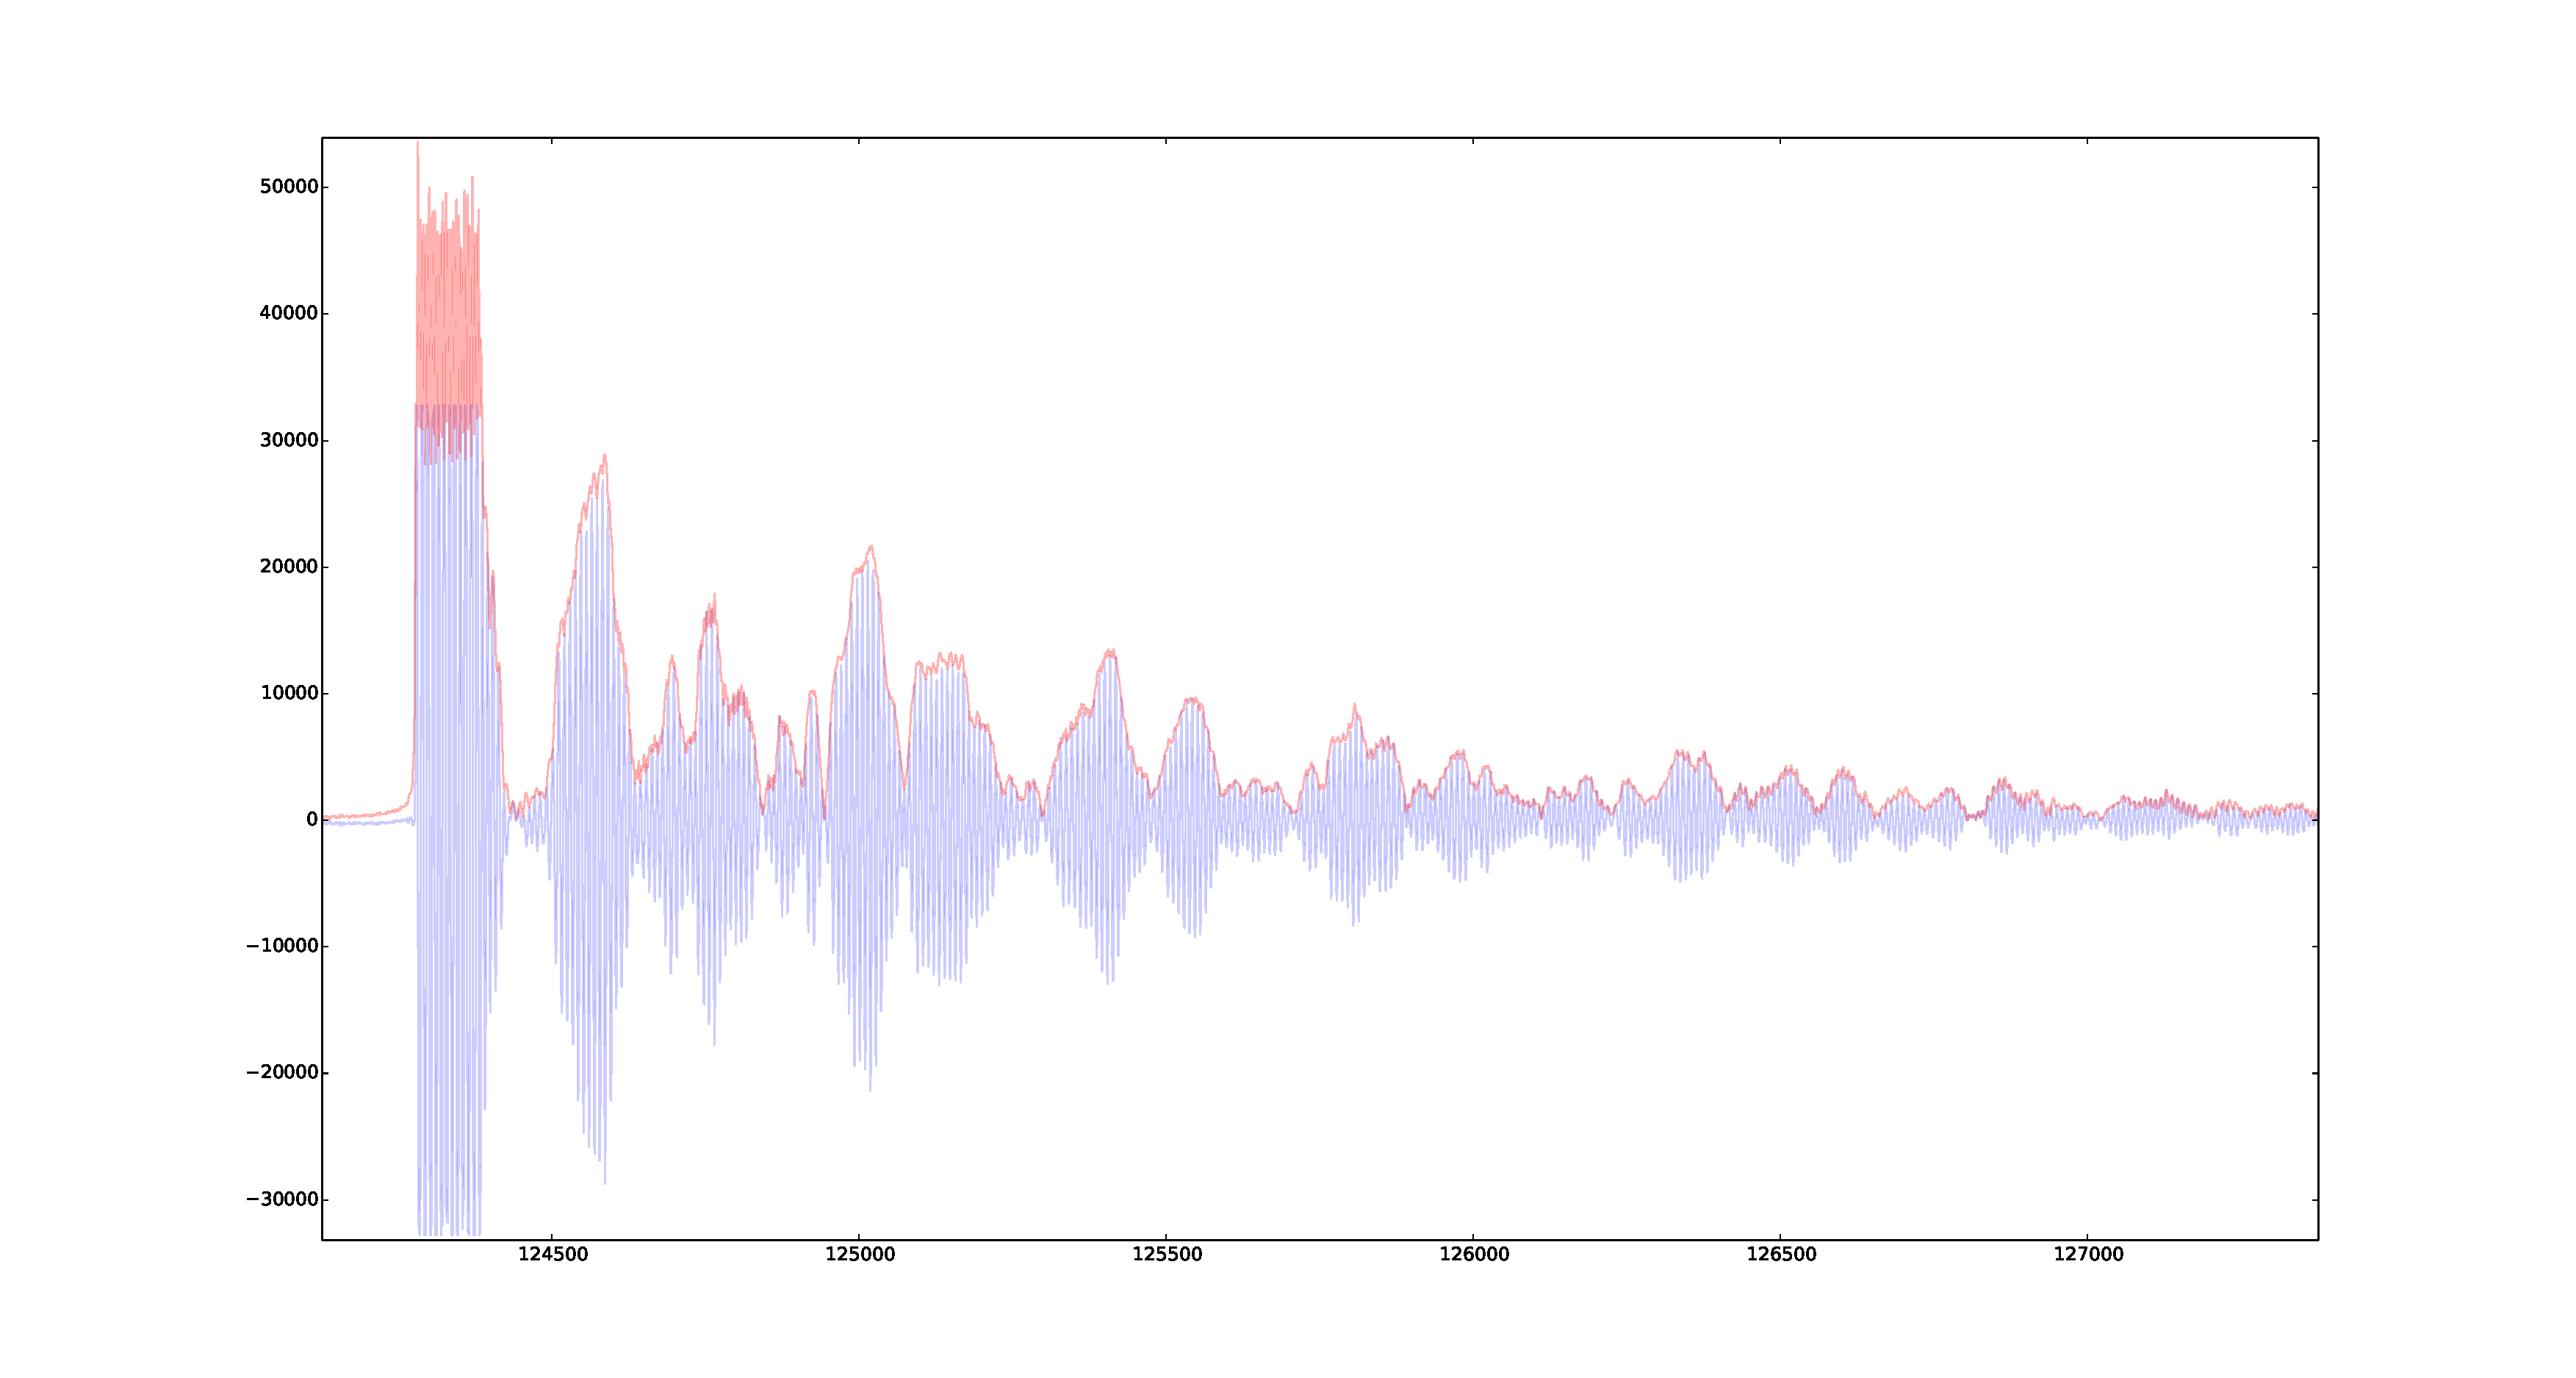
\includegraphics[width=0.45\textwidth]{./fig/inroom.pdf}
\caption{40cm from wall, 5ms chirp}
\end{figure}



% \subsubsection{Phase Diff}



% \subsubsection{Shape of Echo}


% \subsubsection{Iterative Audio Reduction}

% We remove the acoustic effects of an object after determining its existence, and 
% in turn investigate the remaining sound iteratively. 


\subsection{Orientations of All Echoes}

We use TDoA of envelops to different microphones to determine the direction 
of the object represented by the envelop.


Binaural beat


\subsection{Environment Transition Detection}


The pattern of echoes will have a sudden change when walking through a door or corner.

\subsubsection{Spatial Environment Pattern}

